% 第 12 题（4）解析：T²-m 图像（pgfplots，数据描点 + 线性拟合）
% 数据来自题表 6 组测量值；拟合直线 T² = 0.402 + 3.99 m；
% 由 T²=0.880 反查 m=0.120 kg（虚线标出）
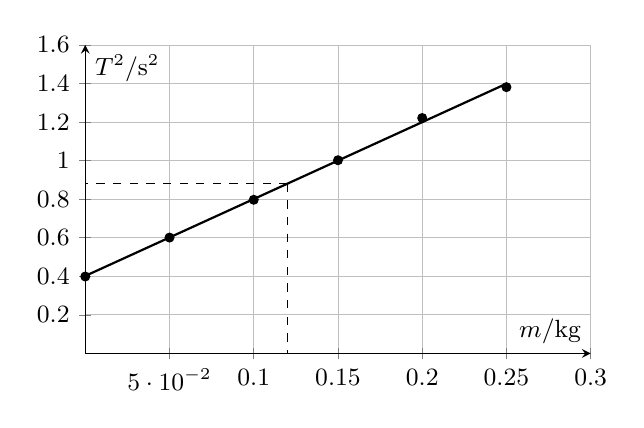
\begin{tikzpicture}
  \begin{axis}[
      width=8cm, height=5.5cm,
      axis lines=middle,
      xlabel={$m$/kg}, ylabel={$T^2$/s$^2$},
      xmin=0, xmax=0.3, ymin=0, ymax=1.6,
      xtick={0,0.05,0.10,0.15,0.20,0.25,0.30},
      ytick={0,0.2,0.4,0.6,0.8,1.0,1.2,1.4,1.6},
      grid=both, grid style={line width=0.3pt, draw=gray!50},
      font=\small]
    \addplot[only marks, mark=*, mark size=1.6pt] coordinates {
      (0.000,0.399) (0.050,0.601) (0.100,0.797)
      (0.150,1.002) (0.200,1.221) (0.250,1.381)};
    \addplot[thick] coordinates {(0,0.402) (0.25,1.399)};
    \draw[dashed] (0.120,0.880) -- (0.120,0) node[below] {\small $0.120$};
    \draw[dashed] (0.120,0.880) -- (0,0.880) node[left] {\small $0.880$};
  \end{axis}
\end{tikzpicture}
